\documentclass[serif,mathserif, 12pt]{beamer}
\usepackage{etex}
\usepackage{amsmath, amsfonts, epsfig, xspace}
\usepackage{algorithm,algorithmic}
\usepackage{pstricks,pst-node}
\usepackage{multimedia}
\usepackage[normal,tight,center]{subfigure}
\setlength{\subfigcapskip}{-.5em}
\usepackage{tkz-euclide}
\usetkzobj{all}
\usepackage{beamerthemesplit}
\usetheme{lankton-keynote}
\usepackage{graphicx,color}
% remove caption of figure
\usepackage[labelformat=empty]{caption}

\usepackage[none]{hyphenat} % hyphenation is ugly in slides
\usepackage{parskip}

\usepackage{relsize} % \smaller to change size

\usepackage{tikz}
\usetikzlibrary{calc}

\usetikzlibrary{arrows}

\newcommand{\TikzDraw}[2][]{
  \begin{tikzpicture}[overlay, remember picture, shift={(current page.center)}, #1]
    #2
  \end{tikzpicture}
}

\newcommand{\gridlines}{
  \TikzDraw{
    \draw[help lines,xstep=.2,ystep=.2,red!20] (current page.south west) grid (current page.north east);
    \draw[help lines,xstep=1,ystep=1,red] (current page.south west) grid (current page.north east);
    \foreach \x in {-15,-14,...,15} {
      \node [anchor=north, red] at (\x,0) {\tiny \x};
      \node [anchor=east,red] at (0,\x) {\tiny \x};
    }
  }
}

\newcommand{\DrawOnImg}[3][]
{
  \begin{tikzpicture}
    \node[anchor=south west,inner sep=0] (image) at (0,0){
      #2
    };
    \begin{scope}[x={(image.south east)},y={(image.north west)}]
      \ifthenelse{\equal{#1}{grid}}
                 {\draw[color=blue, style=dashed] (0,0) grid[xstep=.1, ystep=.1] (1.0001,1.0001);}
                 {}
                 #3
    \end{scope}
  \end{tikzpicture}
}

\usetikzlibrary{matrix}

\newcommand{\BOLD}[1]{\mathbf{#1}}
\newcommand{\BOLDG}[1]{\boldsymbol{#1}}
\newcommand{\PDIF}[2]{\frac{\partial #1}{\partial #2}}
\newcommand{\TODO}[1]{\textcolor{red}{#1}}
\newcommand{\TODOB}[1]{\textcolor{blue}{#1}}
\newcommand{\TODOG}[1]{\textcolor{green!50!black}{#1}}
\newcommand{\argmin}{\operatornamewithlimits{arg\min}}
\DeclareMathOperator{\tr}{tr}
\DeclareMathOperator{\cond}{cond}
\DeclareMathOperator{\ST}{s.t.}
\DeclareMathOperator{\diag}{diag}
\DeclareMathOperator{\Div}{div}

\input pdf-trans
\newbox\qbox
\def\usecolor#1{\csname\string\color@#1\endcsname\space}
\newcommand\bordercolor[1]{\colsplit{1}{#1}}
\newcommand\fillcolor[1]{\colsplit{0}{#1}}
\newcommand\outline[1]{\leavevmode%
  \def\maltext{#1}%
  \setbox\qbox=\hbox{\maltext}%
  \boxgs{Q q 2 Tr 110 Tz \mythickness\space w \fillcol\space \bordercol\space}{}% m@: 110 Tz is to scale up the horizontal size
  \copy\qbox%
}
\makeatother
\newcommand\colsplit[2]{\colorlet{tmpcolor}{#2}\edef\tmp{\usecolor{tmpcolor}}%
  \def\tmpB{}\expandafter\colsplithelp\tmp\relax%
  \ifnum0=#1\relax\edef\fillcol{\tmpB}\else\edef\bordercol{\tmpC}\fi}
\def\colsplithelp#1#2 #3\relax{%
  \edef\tmpB{\tmpB#1#2 }%
  \ifnum `#1>`9\relax\def\tmpC{#3}\else\colsplithelp#3\relax\fi
}
\bordercolor{black}
\fillcolor{white}
\def\mythickness{.28}

\title[\hspace{2em}\insertframenumber/\inserttotalframenumber]{
  Multiresolution Analysis and Operator-adapted Wavelet
}
\date{May 10, 2019}

\author{Jiong Chen}

\makeatletter
\let\@@magyar@captionfix\relax
\makeatother

\begin{document}

\maketitle

\begin{frame}
  \frametitle{Finite element analysis}
  \begin{itemize}
  \item Consider linear problem
    \[
    \mathcal{L}u = g,
    \]
  \item $\mathcal{L}: H\rightarrow H^s$, continuous, linear, bijective, self-adjoint positive-definite operator.
  \item Solve by weak form
    \[
    \langle u, v \rangle_\mathcal{L} = \langle g, v\rangle_{L^2}
    \]
  \item FEM: $u, v$ are so called basis functions.
  \end{itemize}
\end{frame}

\begin{frame}
  \frametitle{Wavelet Galerkin approach}
  \begin{itemize}
  \item Finite dimensional approximation
    \[
    H \approx \mathcal{V}^q
    \]
  \item Nested functional space
    \[
      \mathcal{V}^k\subset \mathcal{V}^{k+1}, k = 1\dots q-1
    \]
  \item \TODO{Orthogonal decomposition}
    \[
    \begin{split}
      &\mathcal{V}^{k+1} = \mathcal{V}^k \oplus \mathcal{W}^k, k = 1\dots q-1 \\
      &H\approx \mathcal{V}^q = \mathcal{V}^1 \oplus \mathcal{W}^1
      \oplus \mathcal{W}^2 \oplus \dots \oplus \mathcal{W}^{q-2} \oplus
      \mathcal{W}^{q-1}
    \end{split}    
    \]
  \end{itemize}
  \TikzDraw {
    \node at (0, 0) {
      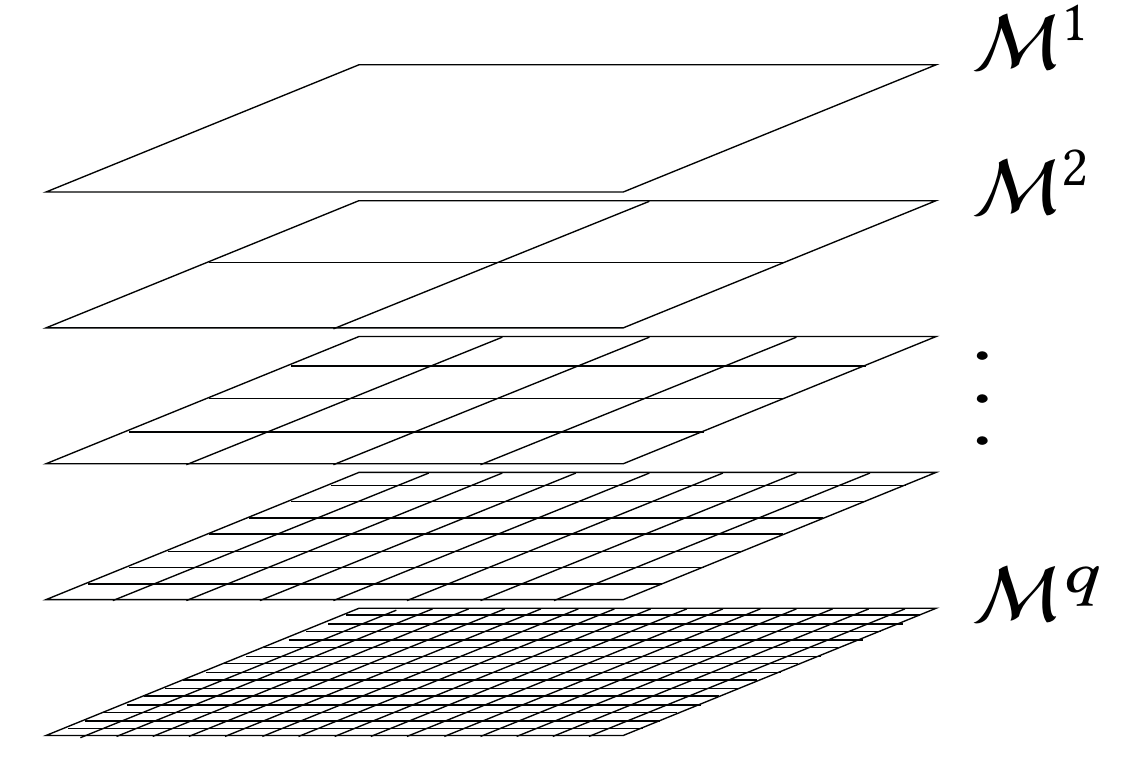
\includegraphics[width=0.2\textwidth]{img/nested_mesh}
    };
  }
\end{frame}

\begin{frame}
  \frametitle{Wavelet Galerkin approach}
  \begin{itemize}
  \item Parameterization
    \[
    \begin{split}
    &\underbrace{\mathcal{V}^{k+1}}_{\{\varphi_i^{k+1}\}_{i=1}^{n_{k+1}}}
    =\underbrace{\mathcal{V}^k}_{\{\varphi_i^k\}_{i=1}^{n_k}} \oplus
    \underbrace{\mathcal{W}^k}_{\{\psi_i^k\}_{i=1}^{N_k=n_{k+1}-n_k}} \\
    &u^q = \sum_{i=1}^{n_1} v_i^1 \varphi_i^1
    + \sum_{k=1}^{q-1}\sum_{j=1}^{N_k} w_j^k \psi_j^k
    \end{split}
    \]
  \item Discretized linear weak form eqn $Lw = g$
    \[
    L =
    \begin{pmatrix}
      A^1 & M^{(1, 2)} & \dots & M^{(1, q)} \\
      M^{(2, 1)} & B^1 & \dots & M^{(2, q)} \\
      \vdots & \vdots &\ddots & \vdots \\
      M^{(q-1, 1)} & M^{(q, 2)} &\dots & B^{q-1}
    \end{pmatrix}
    \]
  \end{itemize}
\end{frame}

\begin{frame}
  \frametitle{$\mathcal{L}$-orthogonality}
  \begin{itemize}
  \item Why $L2$ implies a good decomposition?
  \item \TODO{\emph{Scale-orthogonal wavelets}}
    \begin{itemize}
    \item[-] be operator-orthogonal to block-diagonalize the $L$
    \item[-] produce well-conditioned stiffness matrices
    \item[-] be localized or have fast decay
    \end{itemize}
  \item $\mathcal{L}$-orthogonality
    \[
    \begin{split}
      &\mathcal{\outline{V}}^{k+1} = \mathcal{\outline{V}}^k \oplus_\mathcal{L} \mathcal{\outline{W}}^k \\
      &H\approx \mathcal{V}^q = \mathcal{\outline{V}}^1 \oplus_\mathcal{L} \mathcal{\outline{W}}^1
      \oplus_\mathcal{L} \mathcal{\outline{W}}^2 \oplus_\mathcal{L} \dots \oplus_\mathcal{L} \mathcal{\outline{W}}^{q-2} \oplus_\mathcal{L}      \mathcal{\outline{W}}^{q-1}
    \end{split}
    \]
  \end{itemize}
\end{frame}

\begin{frame}
  \frametitle{$\mathcal{L}$-orthogonality}
  \begin{itemize}
  \item Stiffness
    \[
    \begin{split}
    &L =
    \begin{pmatrix}
      \outline{A}^1 & 0 & \dots & 0 \\
       0 & \outline{B}^1 & \dots & 0 \\
      \vdots & \vdots &\ddots & \vdots \\
      0 & 0 &\dots & \outline{B}^{q-1}
    \end{pmatrix}
    \\
    &\outline{A}^1_{i, j} = \langle \outline{$\varphi$}_i^1, \outline{$\varphi$}_j^1
    \rangle_\mathcal{L}, \quad \outline{B}^k_{i, j} = \langle \outline{$\psi$}_i^k, \outline{$\psi$}_j^k
    \rangle_\mathcal{L} \\ 
    \end{split}
    \]
  \item Independent linear systems
    \begin{equation*}
      \begin{cases}
        \outline{A}^1 v^1 = \outline{a}^1, \\
        \outline{B}^k w^k = \outline{b}^k, k =1\dots q-1
      \end{cases}
    \end{equation*}
  \end{itemize}
\end{frame}

\begin{frame}
  \frametitle{Eigen functions}
  \begin{itemize}
  \item Diagonalize stiffness matrix
    \[
    \begin{split}
    &\langle \phi_i, \phi_i \rangle_\mathcal{L} = \lambda_i, \\
    &\langle \phi_i, \phi_j \rangle_\mathcal{L} = 0, i\neq j.
    \end{split}
    \]
  \item Operator-adapted basis: in between of FEM basis and eigen basis
    \begin{itemize}
    \item[-] capture eigenspaces
    \item[-] spatially localized
    \end{itemize}
  \end{itemize}
\end{frame}

\begin{frame}
  \frametitle{Construction}
  \begin{itemize}
  \item How to construct?
  \item Basis refinement
    \[
    \varphi_i^k = \sum_{j=1}^{n_{k+1}}C_{ij}^k\varphi_j^{k+1}
    \]
  \item Wavelet
    \[
    \psi_i^k = \sum_{j=1}^{n_{k+1}}W_{ij}^k\varphi_j^{k+1}
    \]
  \end{itemize}
  \TikzDraw {
    \node at (4, 0) {
      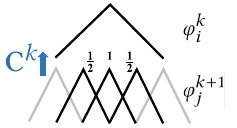
\includegraphics[width=0.3\textwidth]{img/refinement}
    };
  }
\end{frame}

\begin{frame}
  \frametitle{Operator-adapted wavelet}
  \begin{itemize}
  \item Operator-adapted refinability
    \[
    \outline{$\varphi$}_i^k = \sum_{j=1}^{n_{k+1}}\outline{C}_{ij}^k
    \outline{$\varphi$}_j^{k+1}
    \]
  \item Operator adapted wavelets
    \[
    \outline{$\psi$}_i^k = \sum_{j=1}^{n_{k+1}}W_{ij}^k
    \outline{$\varphi$}_j^{k+1}
    \]
  \item $\mathcal{L}$-orthogonality
    \[
    \langle \outline{$\varphi$}_i^k, \outline{$\psi$}_j^k\rangle_\mathcal{L} = 0
    \Rightarrow \outline{C}^k\outline{A}^{k+1}W^{k, T} = 0
    \]
  \TODO{Approximating eigenspaces}
  \end{itemize}  
\end{frame}

\begin{frame}
  \frametitle{Collocation condition}
  \begin{itemize}
  \item Collocation condition
    \[
    \langle \outline{$\varphi$}_i^k, \varphi_j^k\rangle_{L^2} = \delta_{ij}
    \Rightarrow \outline{C}^kC^{k, T } = \mathbb{I}
    \]
  \end{itemize}
  \TODO{Spatially localized}
\end{frame}

\begin{frame}
  \frametitle{Variational formulation}
  \begin{itemize}
  \item Equivalent variational formulation
    \[
    \outline{$\varphi$}_i^k = \argmin_{\outline{$\phi$}\in H} \|
    \outline{$\phi$}\|_\mathcal{L}^2,\quad \ST
    \langle \outline{$\phi$}_i^k, \varphi_j^k\rangle_{L^2}= \delta_{ij}
    \]
  \item Discrete formulation
    \[
    \outline{C}^k = \argmin_{\outline{X}} \tr(\outline{X}\outline{A}^{k+1}
    \outline{X}), \quad \ST \outline{X}C^{k,T} = \mathbb{I}
    \]
  \end{itemize}
\end{frame}

\begin{frame}
  \frametitle{Properties}
  \begin{itemize}
  \item $\cond(\outline{B}^k)$ are uniformly bounded.
  \item $\outline{$\varphi$}_i^k$ decays exponentially fast.
  \item Operator-adapted basis already exhibits very good coarse-graining property.
  \end{itemize}
\end{frame}

\begin{frame}
  \frametitle{}
    \TikzDraw {
    \node at (0, 0.5) {\Huge{Results}};
  }
\end{frame}

\begin{frame}
  \frametitle{}
  \begin{figure}[t]
    \centering
    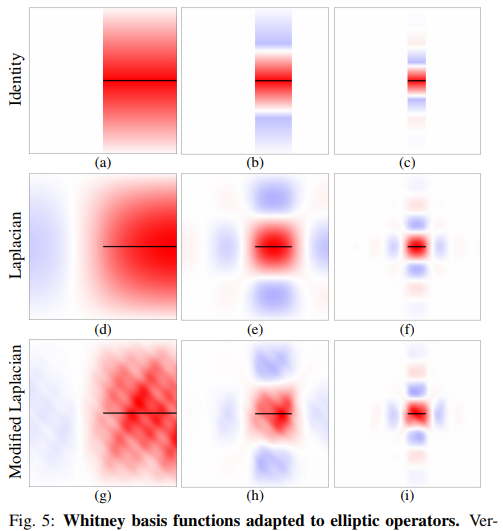
\includegraphics[width=0.75\textwidth]{img/basis_heatmap}
  \end{figure}
\end{frame}

\begin{frame}
  \frametitle{}
  \begin{figure}[t]
    \centering
    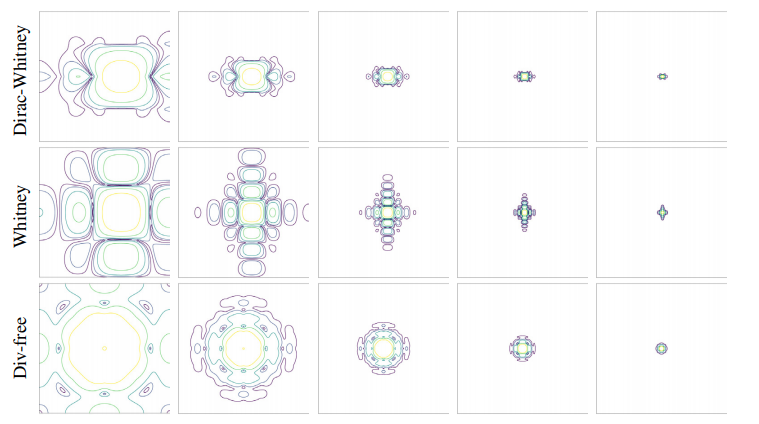
\includegraphics[width=\textwidth]{img/basis_contour}
  \end{figure}
\end{frame}

\begin{frame}
  \frametitle{}
  \begin{figure}[t]
    \centering
    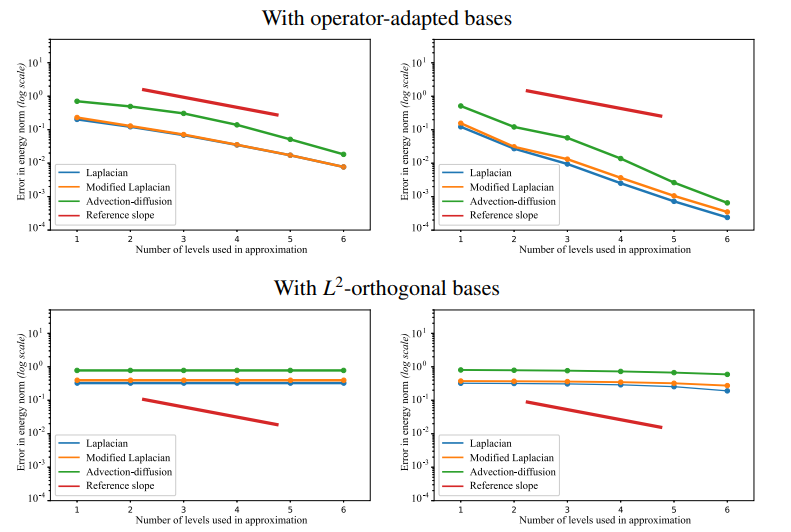
\includegraphics[width=\textwidth]{img/homo_effect}
  \end{figure}
\end{frame}

\begin{frame}
  \frametitle{}
  \begin{figure}[t]
    \centering
    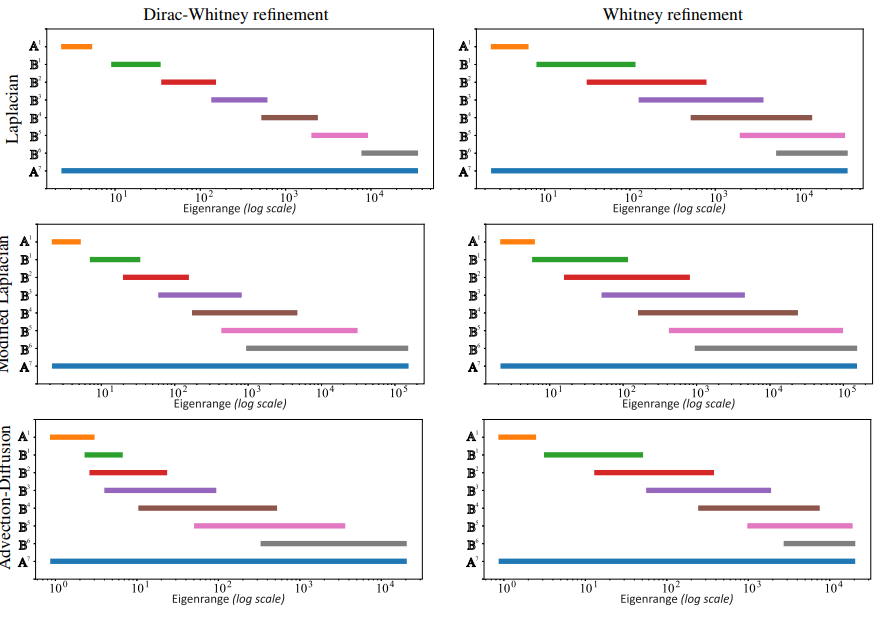
\includegraphics[width=\textwidth]{img/eigen_range}
  \end{figure}
\end{frame}

\begin{frame}
  \frametitle{Future work}
  \begin{itemize}
  \item Multiresolution analysis of space-timing problem
  \item Combine with [Chen 2018]
  \end{itemize}
\end{frame}

\begin{frame} 
  \TikzDraw {
    \node at (0, 0.5) {\Huge{Thanks!}};
  }
  %\gridlines
\end{frame}

\end{document}
